\documentclass{article}
\usepackage{graphicx}
\usepackage{amsfonts}
\usepackage{amsmath}
\usepackage{amsthm}
\usepackage{bigfoot}
\usepackage{booktabs}
\usepackage{hyperref}
\usepackage{cleveref}
\usepackage{mathtools}
\usepackage{siunitx}
\usepackage{changes}

\usepackage{subcaption}
\usepackage{todonotes}
\usepackage{upgreek}
\usepackage{xcolor}

\usepackage{fullpage}
\usepackage[modulo]{lineno}
\linenumbers

\title{LLR 2026: Lab 1 Report}
\author{Valentina Schüller}
\date{\today}

\begin{document}

\maketitle

The code is available at
\url{https://github.com/valentinaschueller/LowRankMethods}.
In the report, I only cover the questions that explicitly required a
plot or discussion.
The remaining exercises are solved in the code in \verb|src/lab1.jl|.

\paragraph{Part 1, Ex. 2.3: Explain why the loop is guaranteed to
  terminate with \(r \geq 1\) for
any \(TOL \geq 0\).}
The loop is guaranteed to terminate since we implemented the
truncation routine in Ex.~1.3 with the condition that at least one
singular triplet is kept in all cases.
That is, even if \(A\) is the zero matrix, \(\sigma_1=0\) will be
preserved by \verb|truncate()|.

\paragraph{Part 2, Ex.~4}
The rank of the first term in the Taylor series, \(T_0=W_0\) is one, by
construction of \(W_0\approx u_0(x,y)\).
For all subsequent Taylor terms, the rank is two.
See \Cref{fig:taylor_sv,fig:taylor_rank} for the corresponding plots:
\Cref{fig:taylor_sv} shows all singular values for \(T_0,\dots,T_7\)
and \Cref{fig:taylor_rank} shows the effective rank (i.e., the number
of singular values larger than \num{e-14}).
\Cref{fig:taylor_sv} already shows that the leading singular values
of the Taylor terms decay with \(k\).
This matches the behavior in \Cref{fig:taylor_frobenius}, which shows
the Frobenius norm of the Taylor terms for increasing \(k\).

Even though the Taylor terms for \(k\geq1\) have rank 2, the Taylor
\emph{series}, \(\sum_{k=0}^\infty T_k\) has rank 1.
This is expected since the solution to the transport problem we solve
should retain its rank.
I numerically show in \Cref{fig:taylor_series_sigma2} how the second
singular value of the partial sums \(\sum_{k=0}^{p}T_k\) decays for
increasing \(p\).
For \(p=0\), \(T_0=W_0\), so \(\sigma_2\approx 0\).
For \(p>0\), \(\sigma_1(T_k)\approx \sigma_2(T_k)\) (cf.
\Cref{fig:taylor_sv}), but it roughly scales with a factor \(\Delta t\)
for each additional Taylor term.
This suggests that we can use, e.g., \(\Delta t^{p-1}\) as a rank
truncation criterion for low-rank approximations.

\begin{figure}[h]
  \centering
  \begin{subfigure}{0.49\textwidth}
    \centering
    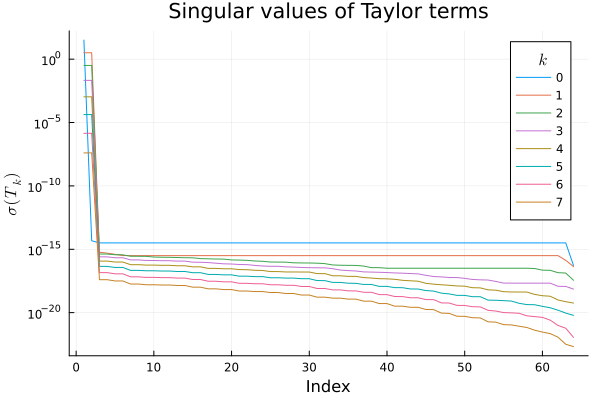
\includegraphics[width=\textwidth]{figures/lab1_taylor_sv.png}
    \caption{\label{fig:taylor_sv}}
  \end{subfigure}
  \hfill
  \begin{subfigure}{0.49\textwidth}
    \centering
    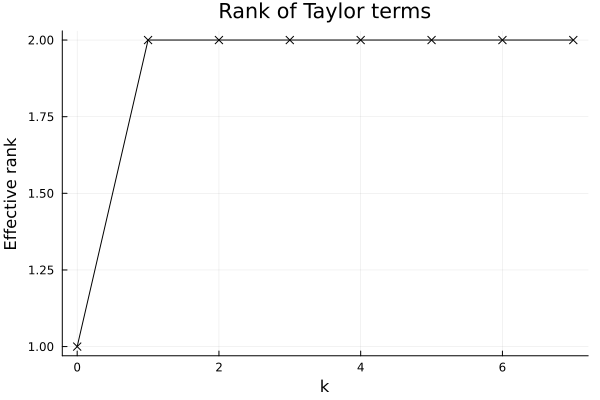
\includegraphics[width=\textwidth]{figures/lab1_taylor_rank.png}
    \caption{\label{fig:taylor_rank}}
  \end{subfigure}
  \begin{subfigure}{0.49\textwidth}
    \centering
    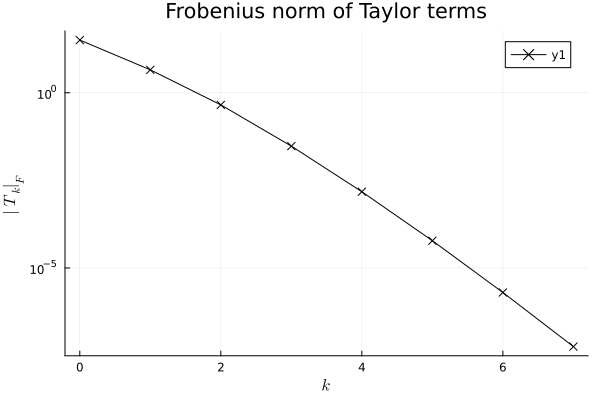
\includegraphics[width=\textwidth]{figures/lab1_taylor_frobenius.png}
    \caption{\label{fig:taylor_frobenius}}
  \end{subfigure}
  \hfill
  \begin{subfigure}{0.49\textwidth}
    \centering
    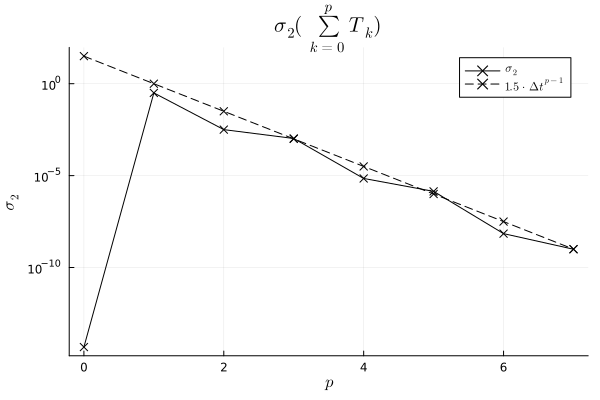
\includegraphics[width=\textwidth]{figures/lab1_taylor_series_sigma2.png}
    \caption{\label{fig:taylor_series_sigma2}}
  \end{subfigure}
  \caption{Plots for Part 2 (Taylor term rank).\label{fig:taylor}}
\end{figure}

\paragraph{Part 3, Ex. 5.3: How does the runtime of \texttt{trunc\_sum}
  scale with \(R\)? At what
point does the thin-QR step dominate over the SVD step?}
I skipped this exercise.

\paragraph{Part 4: Two strategies for the time loop}
\Cref{tab:strategies} reports time to solution and errors for the two
strategies.
Truncating before scaling the Taylor series factors results in
2--5\(\times\) faster simulation at similar errors.
The error (computed as \(e= \|h_x (W_n - W_0)\|_F\)) is roughly
halved when halving
the time step size, as expected.
For some reason, I observed unusually small errors in my third
experiment, for both strategies.

\begin{table}[h]
  \centering
  \begin{tabular}{l|l|l|l|l}
    \(\Delta t\)        & Time (A) & Time (B) & Error (A) & Error (B) \\
    \hline
    \(\Delta t^*\approx0.01\) & 0.14     & 0.62   & 0.22     & 0.22     \\
    \(\Delta t^* / 2\)  & 0.39     & 1.1    & 0.11     & 0.11     \\
    \(\Delta t^* / 4\)  & 0.45     & 2.5    & \num{3.5e-4}   & \num{1.4e-3}   \\
    \(\Delta t^* / 8\)  & 0.89     & 4.9    & \num{2.5e-2}   & \num{2.5e-2}
  \end{tabular}
  \caption{Error and time comparison of strategies A and
  B.\label{tab:strategies}}
\end{table}

\paragraph{Part 5: Solid-body rotation with a Gaussian blob}
For the implementation of part 5, I reused large parts of my
implementation for part 4 and only adapted the differentiation
operators: see \verb|rotation.jl| in the code.
I verified at first that I get the expected rotation behavior with a
full rank solver.
I also verified that the low rank solver matches well with the full
rank solver at \(t=0\) (Ex. 9).

However, I did not manage to implement a stable low rank solver for
this example.
\Cref{fig:solid_body_full,fig:solid_body_lowrank} show the solid body
after one second with the full and the low rank solver, respectively.
The instability in the low rank solver grows over time, leading to
artificial oscillations and a slowed down rotation, see
\Cref{fig:solid_body_lowrank_T}.
In line with this, the numerical rank of the solution in the low rank
solver uniformly grows over the course of the simulation, see
\Cref{fig:solid_body_rank}.

\begin{figure}
  \centering
  \begin{subfigure}{0.49\textwidth}
    \centering
    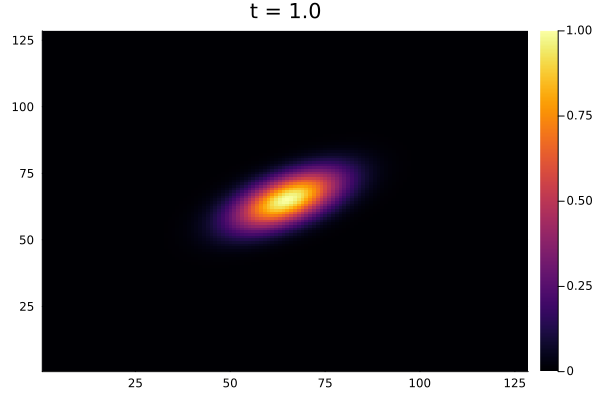
\includegraphics[width=\textwidth]{figures/lab1_fullrank.png}
    \caption{\label{fig:solid_body_full}}
  \end{subfigure}
  \hfill
  \begin{subfigure}{0.49\textwidth}
    \centering
    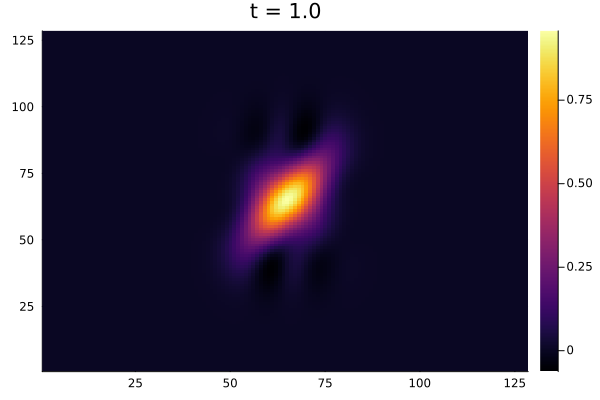
\includegraphics[width=\textwidth]{figures/lab1_lowrank.png}
    \caption{\label{fig:solid_body_lowrank}}
  \end{subfigure}
  \hfill
  \begin{subfigure}{0.49\textwidth}
    \centering
    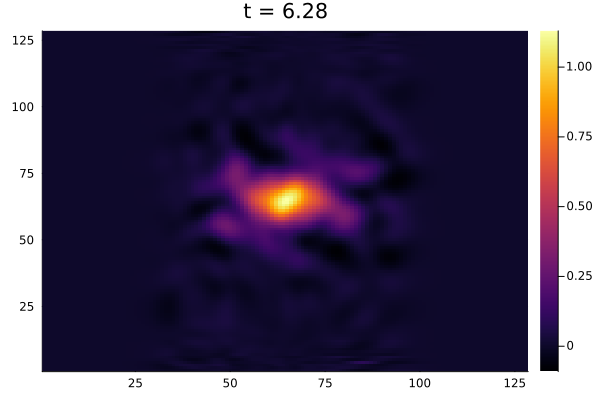
\includegraphics[width=\textwidth]{figures/lab1_llr_fulltime.png}
    \caption{\label{fig:solid_body_lowrank_T}}
  \end{subfigure}
  \hfill
  \begin{subfigure}{0.49\textwidth}
    \centering
    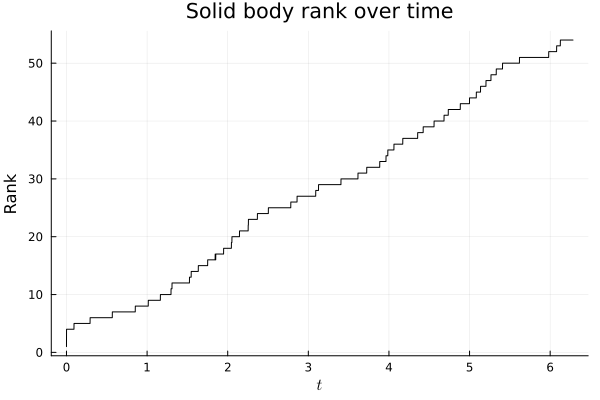
\includegraphics[width=\textwidth]{figures/lab1_lowrank_over_time.png}
    \caption{\label{fig:solid_body_rank}}
  \end{subfigure}
  \hfill
  \caption{Plots for Part 5 (Solid body rotation).}
\end{figure}

\end{document}
